\documentclass[aspectratio=169]{beamer}

\usetheme{Madrid}

\usepackage[utf8]{inputenc}
\usepackage[T1]{fontenc}
\usepackage[brazil]{babel}
\usepackage{amsmath,amssymb,amsfonts}
\usepackage{graphicx}
\usepackage{tikz}
\usepackage[most]{tcolorbox}
\usepackage{pgfplots}
\pgfplotsset{compat=1.18}
\usetikzlibrary{calc}

%-------------------------------------------------
% Cores padrão
%-------------------------------------------------
\definecolor{myblue}{RGB}{0,86,125}
\definecolor{mycyan}{RGB}{0,183,235}
\definecolor{myred}{RGB}{160,30,30}
\definecolor{mygray}{RGB}{245,247,250}
\definecolor{mydark}{RGB}{20,35,45}

\setbeamercolor{structure}{fg=myblue}
\setbeamercolor{frametitle}{bg=myblue,fg=white}
\setbeamercolor{title}{fg=white}

%-------------------------------------------------
% Boxes padrão
%-------------------------------------------------
\newtcolorbox{mybox}[1]{
colback=mygray,
colframe=myblue,
title=#1,
fonttitle=\bfseries,
arc=3mm,
boxrule=0.8pt
}

\newtcolorbox{eqbox}{
colback=white,
colframe=mycyan,
arc=3mm,
boxrule=0.8pt
}

%-------------------------------------------------
% Figura com placeholder
%-------------------------------------------------
%-------------------------------------------------
% Capa de seção
%-------------------------------------------------
\newcommand{\sectioncover}[1]{
\begin{frame}[plain]
\begin{tikzpicture}[remember picture,overlay]
\fill[myblue] (current page.south west) rectangle (current page.north east);
\fill[mycyan,opacity=0.25] (current page.north east) circle (4cm);
\fill[mycyan,opacity=0.18] (current page.south west) circle (5cm);
\end{tikzpicture}
\vfill
\begin{center}
{\color{white}\Huge\bfseries #1}
\end{center}
\vfill
\end{frame}
}

% Definido acima. Este bloco duplicado foi mantido como comentario para evitar
% redefinicao de comando durante a compilacao.
% \newcommand{\sectioncover}[1]{
% \begin{frame}[plain]
% \begin{tikzpicture}[remember picture,overlay]
% \fill[myblue] (current page.south west) rectangle (current page.north east);
% \fill[mycyan,opacity=0.25] (current page.north east) circle (4cm);
% \fill[mycyan,opacity=0.18] (current page.south west) circle (5cm);
% \end{tikzpicture}
% \vfill
% \begin{center}
% {\color{white}\Huge\bfseries #1}
% \end{center}
% \vfill
% \end{frame}
% }
%
% Trecho solto de uma macro anterior, comentado para nao quebrar o preambulo:
% {\scriptsize #3}
% \end{center}
% }


\newcommand{\notas}[1]{%
\begin{tikzpicture}[remember picture,overlay]
\node[anchor=south west,
      xshift=3mm,
      yshift=3mm,
      draw,
      rectangle,
      rounded corners=2pt,
      fill=white,
      font=\tiny,
      inner sep=2pt]
at (current page.south west)
	{notas: #1};
\end{tikzpicture}
}
%-------------------------------------------------
% Capa bonita padrão
%-------------------------------------------------
\newcommand{\beautifulcover}{
{
\setbeamertemplate{navigation symbols}{}
\begin{frame}[plain]
\begin{tikzpicture}[remember picture,overlay]
\fill[mydark] (current page.south west) rectangle (current page.north east);

\fill[myblue!70] 
([xshift=-2.5cm,yshift=1.5cm]current page.south west) circle (4.5cm);

\fill[mycyan!45] 
([xshift=2.5cm,yshift=-1.0cm]current page.north east) circle (4.2cm);

\fill[white,opacity=0.05]
([xshift=0.0cm,yshift=0.0cm]current page.center) circle (7.5cm);

\node[align=center,text=white] at (current page.center) {
{\Huge\bfseries Multipolos Elétricos}\\[0.35cm]
{\Large Capítulo 5}\\[0.55cm]
{\large Matéria Condutora}
};

\node[align=center,text=white!75] at ([yshift=-3.1cm]current page.center) {
Prof. Dr. Rafael Camargo Rodrigues de Lima
};
\end{tikzpicture}
\end{frame}
}
}

\begin{document}

\beautifulcover

\begin{frame}[plain]

\begin{tikzpicture}[remember picture,overlay]
\node at (current page.center) {
    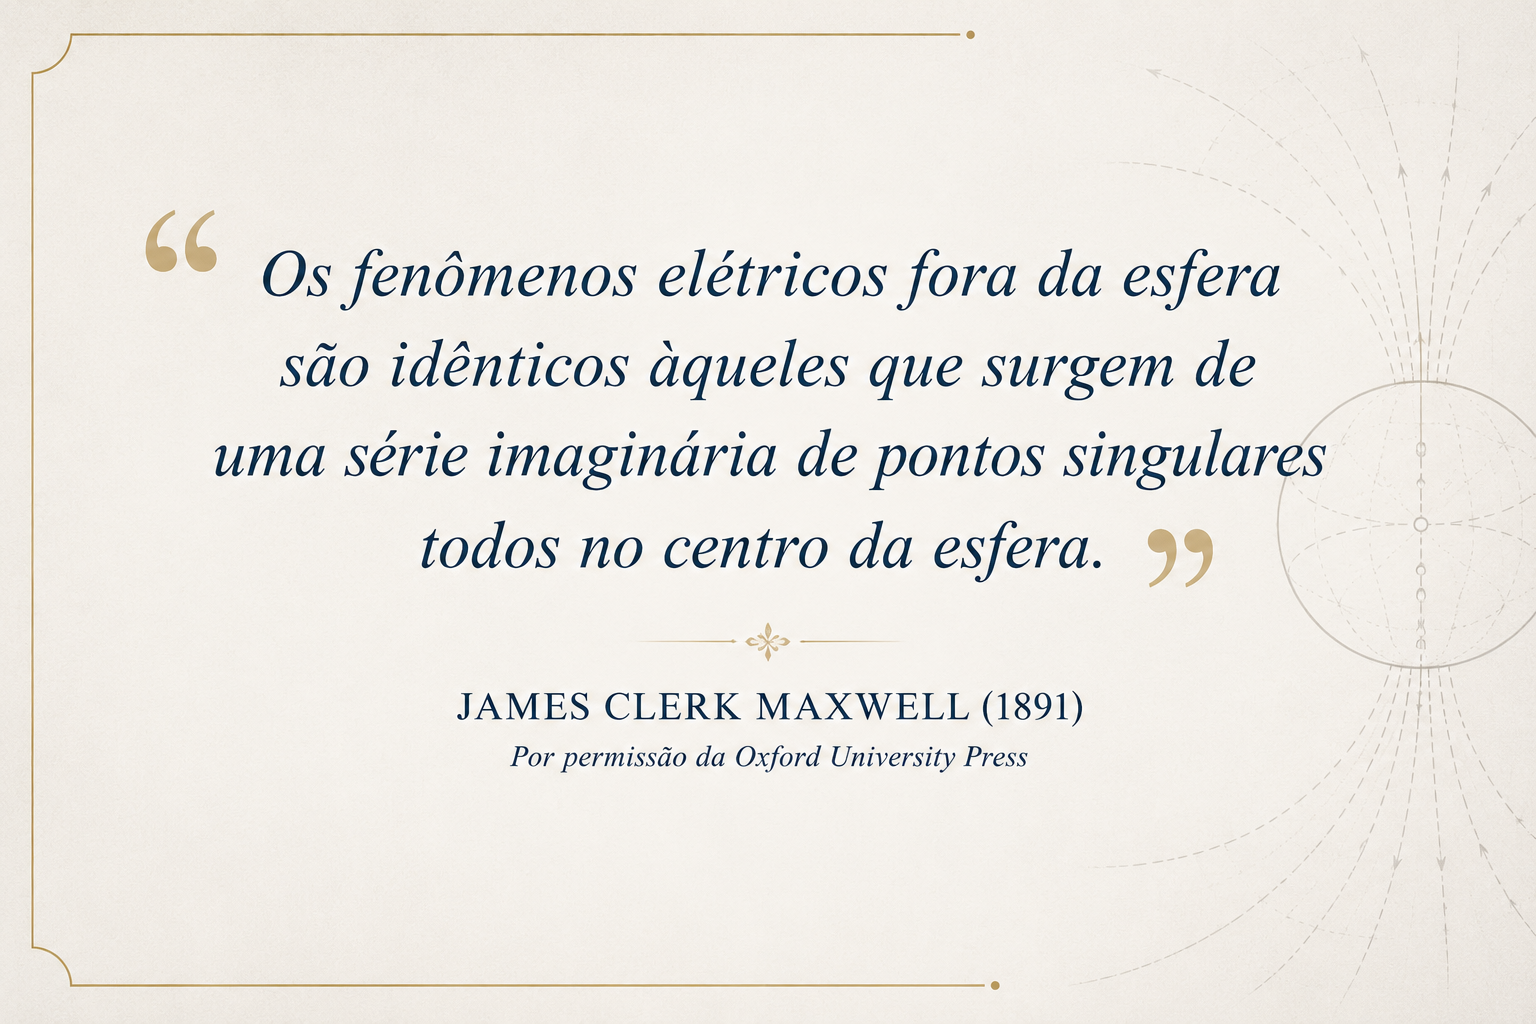
\includegraphics[
        width=\paperwidth,
        height=\paperheight
    ]{ChatGPT Image 12 de mai. de 2026, 08_41_07.png}
};
\end{tikzpicture}

\end{frame}



%-------------------------------------------------
\begin{frame}[plain]
\begin{tikzpicture}[remember picture,overlay]
\fill[myblue] (current page.south west) rectangle (current page.north east);
\fill[mycyan,opacity=0.25] (current page.north east) circle (4cm);
\fill[mycyan,opacity=0.18] (current page.south west) circle (5cm);
\end{tikzpicture}

\vfill
\begin{center}
{\color{white}\Huge\bfseries Matéria Condutora}

\vspace{0.4cm}

{\color{white}\Large Capítulo 5}

\vspace{0.8cm}

{\color{white}\large Condutores perfeitos, indução eletrostática e polarizabilidade}
\end{center}
\vfill
\end{frame}

%-------------------------------------------------
\sectioncover{5.1 Introdução}

%-------------------------------------------------
\begin{frame}{Condutor Perfeito}

\begin{mybox}{Ideia física}
Um \textbf{condutor perfeito} é um modelo macroscópico no qual campos elétricos
estáticos são completamente excluídos do interior do material.
\end{mybox}

\vspace{0.3cm}

Como

\begin{eqbox}
\begin{equation}
\epsilon_0 \nabla \cdot \mathbf E(\mathbf r)=\rho(\mathbf r),
\label{eq:gauss-local}
\end{equation}
\end{eqbox}

segue que, no interior de um condutor perfeito, devemos ter:

\begin{eqbox}
\begin{equation}
\mathbf E(\mathbf r)=0,
\qquad
\rho(\mathbf r)=0,
\qquad
\mathbf r \in V.
\tag{5.1}
\label{eq:condutor-perfeito}
\end{equation}
\end{eqbox}

\end{frame}

%-------------------------------------------------
\begin{frame}{Consequência: a carga fica na superfície}

\begin{mybox}{Resultado central}
Se \(\rho(\mathbf r)=0\) no interior do condutor, qualquer carga líquida em excesso
não pode permanecer distribuída no volume.
\end{mybox}

\vspace{0.3cm}

Portanto, a carga excedente acumula-se na superfície do condutor na forma de uma
densidade superficial:

\[
\sigma(\mathbf r_S).
\]

\begin{alertblock}{Interpretação}
Em equilíbrio eletrostático, o interior do condutor é neutro macroscopicamente,
mas a superfície pode sustentar uma distribuição de carga.
\end{alertblock}

\end{frame}

%-------------------------------------------------
\begin{frame}{Exemplo: esfera condutora isolada}

\begin{columns}

\column{0.45\textwidth}

\begin{mybox}{Esfera condutora}
Considere uma esfera condutora isolada, com:

\begin{itemize}
\item raio \(R\);
\item carga total \(Q\);
\item simetria esférica.
\end{itemize}
\end{mybox}

Pela simetria,

\[
\sigma=\frac{Q}{4\pi R^2}.
\]

\column{0.55\textwidth}

\begin{center}
\begin{tikzpicture}[scale=1.1]
\draw[thick, myblue] (0,0) circle (1.3);
\foreach \ang in {0,30,...,330}{
  \node[myred] at ({1.55*cos(\ang)},{1.55*sin(\ang)}) {\small \(+\)};
}
\draw[->, thick] (0,0) -- (1.3,0) node[midway, above] {\(R\)};
\node at (0,-1.8) {\(\sigma=Q/4\pi R^2\)};
\end{tikzpicture}
\end{center}

\end{columns}

\end{frame}

%-------------------------------------------------
\begin{frame}{Potencial da esfera condutora}

\small

Fora da esfera, pela lei de Gauss, o campo é igual ao de uma carga pontual \(Q\)
no centro:

\[
E(r)=\frac{1}{4\pi\epsilon_0}\frac{Q}{r^2},
\qquad r\ge R.
\]

Logo,

\[
\varphi(r)=\frac{1}{4\pi\epsilon_0}\frac{Q}{r},
\qquad r\ge R.
\]

Dentro do condutor, \(\mathbf E=0\), portanto o potencial é constante.

\begin{eqbox}
\begin{equation}
\varphi(r)=
\begin{cases}
\dfrac{Q}{4\pi\epsilon_0 R},
& r\le R, \\[0.35cm]
\dfrac{Q}{4\pi\epsilon_0 r},
& r\ge R.
\end{cases}
\tag{5.2}
\label{eq:potencial-esfera-condutora}
\end{equation}
\end{eqbox}

\end{frame}

%-------------------------------------------------
\sectioncover{5.2 Indução Eletrostática}

%-------------------------------------------------
\begin{frame}{Ideia de Cavendish}

\begin{mybox}{Campo externo aplicado}
Na presença de um campo externo \(\mathbf E_{\rm ext}\), as cargas móveis do condutor
se rearranjam até que o campo total no interior seja nulo.
\end{mybox}

\begin{eqbox}
\begin{equation}
\mathbf E(\mathbf r)
=
\mathbf E_{\rm ext}(\mathbf r)
+
\mathbf E_{\rm self}(\mathbf r)
=
0,
\qquad
\mathbf r\in V.
\label{eq:campo-total-zero}
\end{equation}
\end{eqbox}

\begin{alertblock}{Nome do fenômeno}
Esse rearranjo de cargas é chamado de \textbf{indução eletrostática}.
\end{alertblock}

\end{frame}

%-------------------------------------------------
\begin{frame}{Figura: polarização de um condutor neutro}

\begin{center}
\begin{tikzpicture}[scale=0.9]

% painel a
\node at (-3.2,2.1) {\textbf{(a) Campo externo}};
\foreach \y in {-1.2,-0.6,0,0.6,1.2}{
  \draw[->, thick] (-5,\y) -- (-1.5,\y+0.25);
}
\draw[thick, fill=mygray] plot[smooth cycle] coordinates {(-4,-0.9) (-3.1,-1.1) (-2.5,-0.4) (-2.7,0.7) (-3.6,0.9) (-4.3,0.3)};
\foreach \p in {(-4.0,-0.4),(-3.7,0.3),(-3.4,0.65)}{
  \node at \p {\(-\)};
}
\foreach \p in {(-2.7,-0.3),(-2.6,0.2),(-2.8,0.6)}{
  \node[myred] at \p {\(+\)};
}
\node at (-3.2,-1.7) {\(\mathbf E_{\rm ext}\)};

% painel b
\node at (3.0,2.1) {\textbf{(b) Equilíbrio}};
\foreach \y in {-1.2,-0.6,0,0.6,1.2}{
  \draw[->, thick] (1,\y) .. controls (2.0,\y+0.2) and (2.2,\y-0.6) .. (3.0,\y-0.2)
  .. controls (3.8,\y+0.3) and (4.1,\y+0.2) .. (5,\y+0.4);
}
\draw[thick, fill=mygray] plot[smooth cycle] coordinates {(2,-0.9) (2.9,-1.1) (3.5,-0.4) (3.3,0.7) (2.4,0.9) (1.7,0.3)};
\foreach \p in {(2.0,-0.4),(2.3,0.3),(2.6,0.65)}{
  \node at \p {\(-\)};
}
\foreach \p in {(3.3,-0.3),(3.4,0.2),(3.2,0.6)}{
  \node[myred] at \p {\(+\)};
}
\node[fill=white] at (2.75,0.0) {\(\mathbf E=0\)};

\end{tikzpicture}
\end{center}

\begin{mybox}{Interpretação}
O campo externo separa levemente as cargas. A distribuição induzida cria
\(\mathbf E_{\rm self}\), que cancela \(\mathbf E_{\rm ext}\) no interior.
\end{mybox}

\end{frame}

%-------------------------------------------------
\begin{frame}{Campo produzido pela carga superficial}

\small

A carga induzida na superfície gera um campo próprio:

\[
\mathbf E_{\rm self}(\mathbf r)
=
\frac{1}{4\pi\epsilon_0}
\int_S dS'\,
\sigma(\mathbf r')
\frac{\mathbf r-\mathbf r'}{|\mathbf r-\mathbf r'|^3}.
\]

Assim, a condição de equilíbrio dentro do condutor fica:

\begin{eqbox}
\begin{equation}
\mathbf E(\mathbf r)
=
\mathbf E_{\rm ext}(\mathbf r)
+
\frac{1}{4\pi\epsilon_0}
\int_S dS'\,
\sigma(\mathbf r')
\frac{\mathbf r-\mathbf r'}{|\mathbf r-\mathbf r'|^3}
=
0,
\qquad
\mathbf r\in V.
\tag{5.3}
\label{eq:campo-superficie-condutor}
\end{equation}
\end{eqbox}

\end{frame}

%-------------------------------------------------
\begin{frame}{Comentário microscópico}

\begin{mybox}{O que realmente se move?}
Em um metal real, a indução eletrostática não exige um deslocamento macroscópico
de elétrons por longas distâncias.
\end{mybox}

\begin{itemize}
\item As funções de onda eletrônicas são perturbadas pelo campo externo.
\item Pequenas redistribuições locais produzem excesso ou déficit de carga na superfície.
\item No volume, a média macroscópica da carga perturbada é zero.
\end{itemize}

\begin{alertblock}{Resumo}
A indução é um fenômeno macroscópico, mas sua origem está em pequenas
perturbações microscópicas das cargas móveis.
\end{alertblock}

\end{frame}

%-------------------------------------------------
\begin{frame}{Momento de dipolo induzido}

\small

Para um condutor neutro em um campo externo uniforme, a distribuição superficial
induzida pode produzir, longe do condutor, um campo aproximadamente dipolar.

\begin{eqbox}
\begin{equation}
\mathbf p
=
\int_S dS\,
\mathbf r\,\sigma(\mathbf r).
\tag{5.4}
\label{eq:dipolo-induzido}
\end{equation}
\end{eqbox}

\begin{mybox}{Interpretação}
O momento de dipolo mede a separação efetiva entre regiões de excesso e déficit
de carga induzida.
\end{mybox}

Para objetos não esféricos, também aparecem contribuições de quadrupolo e
multipolos superiores.

\end{frame}

%-------------------------------------------------
\sectioncover{Teorema de Thomson}

%-------------------------------------------------
\begin{frame}{Teorema de Thomson da Eletrostática}

\begin{mybox}{Enunciado}
A energia eletrostática de um corpo condutor de forma e tamanho fixos é mínima
quando a carga \(Q\) se distribui de modo que o potencial eletrostático seja
constante em todo o corpo.
\end{mybox}

Como

\[
\mathbf E=-\nabla\varphi,
\]

potencial constante implica

\[
\mathbf E=0.
\]

\begin{alertblock}{Conclusão}
O interior de um condutor perfeito em equilíbrio eletrostático é equipotencial.
\end{alertblock}

\end{frame}

%-------------------------------------------------
\begin{frame}{Prova: Energia eletrostática funcional}

\small

Se \(\rho(\mathbf r)\) é a densidade de carga no volume \(V\), e
\(\varphi_{\rm ext}(\mathbf r)\) é o potencial produzido por cargas externas fixas,
a energia eletrostática é:

\begin{eqbox}
\begin{equation}
U_E[\rho]
=
\frac{1}{8\pi\epsilon_0}
\int_V d^3r
\int_V d^3r'\,
\frac{\rho(\mathbf r)\rho(\mathbf r')}
{|\mathbf r-\mathbf r'|}
+
\int_V d^3r\,
\rho(\mathbf r)\varphi_{\rm ext}(\mathbf r).
\tag{5.5}
\label{eq:energia-funcional}
\end{equation}
\end{eqbox}

\begin{mybox}{Observação}
O fator \(1/2\), embutido em \(1/8\pi\epsilon_0\), evita contar duas vezes a
interação entre pares de elementos de carga.
\end{mybox}
\notas{pag. 1-4}
\end{frame}

%-------------------------------------------------
\begin{frame}{Queremos minimizar $U_E$}

\small

A carga total é mantida fixa:

\[
Q=\int_V d^3r\,\rho(\mathbf r).
\]

Para minimizar \(U_E[\rho]\) com essa restrição, usamos um multiplicador de
Lagrange \(\lambda\):

\begin{eqbox}
\begin{equation}
I[\rho]
=
U_E[\rho]
-
\lambda
\int_V d^3r\,\rho(\mathbf r).
\tag{5.6}
\label{eq:funcional-lagrange}
\end{equation}
\end{eqbox}

O extremo da energia ocorre quando:

\begin{eqbox}
\begin{equation}
\delta I
=
I[\rho+\delta\rho]
-
I[\rho]
=
0.
\tag{5.7}
\label{eq:variacao-zero}
\end{equation}
\end{eqbox}

\end{frame}

%-------------------------------------------------
\begin{frame}{Variação do termo de autoenergia}

\small

No termo duplo, fazemos:

\[
\rho(\mathbf r)\to \rho(\mathbf r)+\delta\rho(\mathbf r),
\qquad
\rho(\mathbf r')\to \rho(\mathbf r')+\delta\rho(\mathbf r').
\]

Mantendo apenas termos lineares em \(\delta\rho\):

\begin{eqbox}
\begin{equation}
\delta I
=
\frac{1}{8\pi\epsilon_0}
\int_V d^3r
\int_V d^3r'\,
\left[
\frac{\rho(\mathbf r)\delta\rho(\mathbf r')}
{|\mathbf r-\mathbf r'|}
+
\frac{\delta\rho(\mathbf r)\rho(\mathbf r')}
{|\mathbf r-\mathbf r'|}
\right]
+
\int_V d^3r\,\delta\rho(\mathbf r)\varphi_{\rm ext}(\mathbf r)
-
\lambda
\int_V d^3r\,\delta\rho(\mathbf r).
\tag{5.8}
\label{eq:variacao-I}
\end{equation}
\end{eqbox}

\end{frame}

%-------------------------------------------------
\begin{frame}{Por que aparece o fator 2?}

\small

O primeiro termo dentro dos colchetes pode ser reescrito trocando os nomes das
variáveis mudas:

\[
\mathbf r \leftrightarrow \mathbf r'.
\]

Como

\[
|\mathbf r-\mathbf r'|=|\mathbf r'-\mathbf r|,
\]

os dois termos lineares são iguais. Portanto,

\[
\frac{1}{8\pi\epsilon_0}\times 2
=
\frac{1}{4\pi\epsilon_0}.
\]

Assim,

\begin{eqbox}
\begin{equation}
\delta I
=
\int_V d^3r\,\delta\rho(\mathbf r)
\left[
\frac{1}{4\pi\epsilon_0}
\int_V d^3r'\,
\frac{\rho(\mathbf r')}
{|\mathbf r-\mathbf r'|}
+
\varphi_{\rm ext}(\mathbf r)
-
\lambda
\right].
\tag{5.9}
\label{eq:variacao-fatorada}
\end{equation}
\end{eqbox}

\end{frame}

%-------------------------------------------------
\begin{frame}{Condição de extremo}

\small

Como \(\delta\rho(\mathbf r)\) é arbitrária, o termo entre colchetes deve ser nulo:

\begin{eqbox}
\begin{equation}
\frac{1}{4\pi\epsilon_0}
\int_V d^3r'\,
\frac{\rho(\mathbf r')}
{|\mathbf r-\mathbf r'|}
+
\varphi_{\rm ext}(\mathbf r)
=
\lambda,
\qquad
\mathbf r\in V.
\tag{5.10}
\label{eq:potencial-constante}
\end{equation}
\end{eqbox}

\begin{mybox}{Identificação}
O lado esquerdo é o potencial eletrostático total:

\[
\varphi_{\rm tot}(\mathbf r)
=
\varphi_{\rm self}(\mathbf r)+\varphi_{\rm ext}(\mathbf r).
\]
\end{mybox}

Logo,

\[
\varphi_{\rm tot}(\mathbf r)=\lambda=\text{constante}.
\]

\end{frame}

%-------------------------------------------------
\begin{frame}{Conclusão do teorema de Thomson}

\begin{mybox}{Resultado}
A configuração de equilíbrio minimiza a energia quando o potencial total é
constante no condutor:
\[
\varphi_{\rm tot}=\text{constante}.
\]
\end{mybox}

Como

\[
\mathbf E=-\nabla \varphi_{\rm tot},
\]

segue que

\[
\mathbf E=0
\]

em todo o interior do condutor.

\end{frame}

\begin{frame}
\begin{alertblock}{Comentário}
Os termos de segunda ordem em \(\delta\rho\) são positivos, portanto o extremo é
um mínimo de energia, não um máximo.
\end{alertblock}

\end{frame}

%-------------------------------------------------
\sectioncover{Exemplo 5.1: esfera condutora em campo uniforme}

%-------------------------------------------------
\begin{frame}{Problema}

\begin{mybox}{Exemplo 5.1}
Encontrar o potencial produzido por uma esfera condutora de raio \(R\) colocada
em um campo elétrico uniforme

\[
\mathbf E_0=E_0\hat{\mathbf z}.
\]

Também mostrar que a esfera adquire momento de dipolo

\[
\mathbf p=\alpha\epsilon_0\mathbf E_0,
\qquad
\alpha=4\pi R^3.
\]
\end{mybox}

\end{frame}

%-------------------------------------------------
\begin{frame}{Geometria do problema}

\begin{center}
\begin{tikzpicture}[scale=1.1]

\foreach \y in {-1.2,-0.6,0,0.6,1.2}{
  \draw[->, thick] (-3,\y) -- (3,\y);
}

\draw[thick, fill=white] (0,0) circle (1.2);

\draw[->, thick] (0,0) -- (0.85,0.85);
\node at (0.55,0.25) {\(\theta\)};
\node at (0.65,0.75) {\(R\)};

\foreach \p in {(-0.8,0.7),(-1.0,0.1),(-0.8,-0.6)}{
  \node at \p {\(-\)};
}
\foreach \p in {(0.8,0.7),(1.0,0.1),(0.8,-0.6)}{
  \node[myred] at \p {\(+\)};
}

\node at (0,-1.7) {Esfera condutora};
\node at (2.4,1.55) {\(\mathbf E_0=E_0\hat{\mathbf z}\)};

\end{tikzpicture}
\end{center}

\begin{mybox}{Simetria}
A distribuição induzida depende apenas de \(\theta\), isto é,
\[
\sigma=\sigma(\theta).
\]
\end{mybox}

\end{frame}

%-------------------------------------------------
\begin{frame}{Potencial do campo externo}

\small

Um campo uniforme na direção \(z\) pode ser escrito como:

\[
\mathbf E_0=E_0\hat{\mathbf z}.
\]

Como \(\mathbf E=-\nabla\varphi\), um potencial correspondente é:

\begin{eqbox}
\begin{equation}
\varphi_{\rm ext}(r,\theta)
=
-E_0 z
=
-E_0 r\cos\theta.
\label{eq:potencial-externo-uniforme}
\end{equation}
\end{eqbox}

Dentro da esfera condutora, o campo total deve ser nulo. Portanto,

\[
\mathbf E_{\rm self}=-\mathbf E_0.
\]

Logo, no interior,

\begin{eqbox}
\begin{equation}
\varphi_{\rm self}(r<R,\theta)
=
E_0 z
=
E_0 r\cos\theta.
\label{eq:potencial-self-interior}
\end{equation}
\end{eqbox}

\end{frame}

%-------------------------------------------------
\begin{frame}{Expansão multipolar exterior}

\small

Fora da esfera, o potencial produzido pela carga induzida satisfaz a equação de
Laplace e pode ser escrito como uma expansão multipolar axial:

\begin{eqbox}
\begin{equation}
\varphi_{\rm self}(r>R,\theta)
=
\frac{A}{r}
+
\frac{B}{r^2}\cos\theta
+
\frac{C}{r^3}P_2(\cos\theta)
+\cdots .
\label{eq:expansao-self}
\end{equation}
\end{eqbox}

\begin{mybox}{Simplificação}
A esfera é neutra, portanto não há termo monopolar:
\[
A=0.
\]

A condição de contorno em \(r=R\) tem dependência angular apenas em
\(\cos\theta\). Por isso, os termos \(P_2,P_3,\ldots\) não aparecem.
\end{mybox}

\end{frame}

%-------------------------------------------------
\begin{frame}{Continuidade do potencial em \(r=R\)}

\small

O potencial deve ser contínuo na superfície:

\[
\varphi_{\rm self}(R^-,\theta)
=
\varphi_{\rm self}(R^+,\theta).
\]

Como

\[
\varphi_{\rm self}(R^-,\theta)=E_0R\cos\theta,
\]

e

\[
\varphi_{\rm self}(R^+,\theta)=\frac{B}{R^2}\cos\theta,
\]

temos:

\[
\frac{B}{R^2}=E_0R.
\]

Logo,

\[
B=E_0R^3.
\]

Portanto,

\begin{eqbox}
\begin{equation}
\varphi_{\rm self}(r>R,\theta)
=
\frac{E_0R^3}{r^2}\cos\theta.
\label{eq:self-exterior-esfera}
\end{equation}
\end{eqbox}

\end{frame}

%-------------------------------------------------
\begin{frame}{Potencial total}

\small

Somando o potencial externo com o potencial induzido:

\[
\varphi_{\rm tot}
=
\varphi_{\rm ext}
+
\varphi_{\rm self}.
\]

No interior:

\[
\varphi_{\rm tot}(r<R,\theta)
=
-E_0r\cos\theta
+
E_0r\cos\theta
=
0.
\]

Fora da esfera:

\begin{eqbox}
\begin{equation}
\varphi_{\rm tot}(r>R,\theta)
=
-E_0r\cos\theta
+
\frac{E_0R^3}{r^2}\cos\theta.
\label{eq:potencial-total-esfera}
\end{equation}
\end{eqbox}

Ou seja,

\[
\varphi_{\rm tot}(r>R,\theta)
=
-E_0
\left(
r-\frac{R^3}{r^2}
\right)
\cos\theta.
\]

\end{frame}

%-------------------------------------------------
\begin{frame}{Comparação com o potencial de um dipolo}

\small

O potencial de um dipolo elétrico \(\mathbf p=p\hat{\mathbf z}\) é:

\begin{eqbox}
\begin{equation}
\varphi_{\rm dip}(r,\theta)
=
\frac{1}{4\pi\epsilon_0}
\frac{p\cos\theta}{r^2}.
\label{eq:potencial-dipolo}
\end{equation}
\end{eqbox}

Comparando com

\[
\varphi_{\rm self}(r>R,\theta)
=
\frac{E_0R^3}{r^2}\cos\theta,
\]

obtemos:

\[
\frac{p}{4\pi\epsilon_0}
=
E_0R^3.
\]

Logo,

\begin{eqbox}
\begin{equation}
\mathbf p
=
4\pi\epsilon_0 R^3\mathbf E_0.
\label{eq:dipolo-esfera}
\end{equation}
\end{eqbox}

\end{frame}

%-------------------------------------------------
\begin{frame}{Polarizabilidade da esfera}

\begin{mybox}{Definição}
A polarizabilidade \(\alpha\) é definida por:
\[
\mathbf p=\alpha\epsilon_0\mathbf E_0.
\]
\end{mybox}

Usando

\[
\mathbf p=4\pi\epsilon_0R^3\mathbf E_0,
\]

temos:

\begin{eqbox}
\begin{equation}
\alpha=4\pi R^3.
\label{eq:polarizabilidade-esfera-resumo}
\end{equation}
\end{eqbox}



\end{frame}

\begin{frame}

\begin{eqbox}
\[
\mathbf p=\alpha\epsilon_0\mathbf E_0.
\]
\end{eqbox}

\begin{eqbox}
\begin{equation}
\alpha=4\pi R^3.
\label{eq:polarizabilidade-esfera}
\end{equation}
\end{eqbox}


\begin{alertblock}{Interpretação}
A polarizabilidade de uma esfera condutora cresce com o seu volume.
\end{alertblock}

\end{frame}
%-------------------------------------------------
\begin{frame}{Campo elétrico externo da esfera}

\small

A partir de

\[
\varphi_{\rm tot}(r,\theta)
=
-E_0
\left(
r-\frac{R^3}{r^2}
\right)
\cos\theta,
\]

temos, em coordenadas esféricas:

\[
E_r=-\frac{\partial \varphi}{\partial r},
\qquad
E_\theta=-\frac{1}{r}\frac{\partial \varphi}{\partial \theta}.
\]

Logo,

\begin{eqbox}
\begin{align}
E_r(r,\theta)
&=
E_0
\left(
1+2\frac{R^3}{r^3}
\right)
\cos\theta,
\label{eq:Er-esfera}
\\
E_\theta(r,\theta)
&=
-E_0
\left(
1-\frac{R^3}{r^3}
\right)
\sin\theta.
\label{eq:Etheta-esfera}
\end{align}
\end{eqbox}

\end{frame}

%-------------------------------------------------
\begin{frame}{Carga superficial induzida}

\small

Na superfície \(r=R\),

\[
E_\theta(R,\theta)=0,
\]

como deve ocorrer em um condutor em equilíbrio.

Além disso,

\[
E_r(R,\theta)
=
3E_0\cos\theta.
\]

A condição de contorno para a componente normal do campo é:

\[
E_{\perp}^{\rm fora}
-
E_{\perp}^{\rm dentro}
=
\frac{\sigma}{\epsilon_0}.
\]

Como \(E_{\perp}^{\rm dentro}=0\), temos:

\begin{eqbox}
\begin{equation}
\sigma(\theta)
=
3\epsilon_0E_0\cos\theta.
\label{eq:sigma-esfera-induzida}
\end{equation}
\end{eqbox}

\end{frame}

%-------------------------------------------------
\begin{frame}{Resumo do exemplo da esfera}

\begin{eqbox}
\[
\varphi_{\rm tot}(r<R,\theta)=0.
\]
\[
\varphi_{\rm tot}(r>R,\theta)
=
-E_0
\left(
r-\frac{R^3}{r^2}
\right)
\cos\theta.
\]
\[
\mathbf p=4\pi\epsilon_0R^3\mathbf E_0.
\]
\[
\alpha=4\pi R^3.
\]
\[
\sigma(\theta)=3\epsilon_0E_0\cos\theta.
\]
\end{eqbox}

\end{frame}

%-------------------------------------------------
\sectioncover{5.2.2 Densidade Superficial de Carga}

%-------------------------------------------------
\begin{frame}{Condições de contorno na superfície}

\small

Considere um ponto \(\mathbf r_S\) na superfície do condutor e
\(\hat{\mathbf n}\) a normal externa.

\begin{mybox}{Condições de matching}
A densidade superficial \(\sigma(\mathbf r_S)\) aparece na descontinuidade da
componente normal do campo elétrico:
\end{mybox}

\begin{eqbox}
\begin{align}
\hat{\mathbf n}\times
\left(
\mathbf E_{\rm out}-\mathbf E_{\rm in}
\right)
&=0,
\tag{5.11}
\label{eq:matching-tangencial-condutor}
\\
\hat{\mathbf n}\cdot
\left(
\mathbf E_{\rm out}-\mathbf E_{\rm in}
\right)
&=
\frac{\sigma(\mathbf r_S)}{\epsilon_0}.
\tag{5.12}
\label{eq:matching-normal-condutor}
\end{align}
\end{eqbox}

\begin{alertblock}{Para um condutor perfeito}
\[
\mathbf E_{\rm in}=0.
\]
\end{alertblock}

\end{frame}

%-------------------------------------------------
\begin{frame}{O campo externo é normal à superfície}

\small

Como \(\mathbf E_{\rm in}=0\), a condição tangencial implica:

\begin{eqbox}
\begin{equation}
\hat{\mathbf n}\times \mathbf E_{\rm out}\big|_S=0.
\tag{5.13}
\label{eq:campo-tangencial-zero-superficie}
\end{equation}
\end{eqbox}

Portanto, imediatamente fora do condutor, o campo não pode ter componente
tangencial.

\begin{center}
\begin{tikzpicture}[scale=1.0]
\fill[mygray] (-3,-0.6) rectangle (3,0);
\draw[thick,myblue] (-3,0) -- (3,0);
\node[anchor=east] at (-3.1,-0.3) {\small condutor};
\node[anchor=east] at (-3.1,0.45) {\small exterior};

\foreach \x in {-2.2,-1.1,0,1.1,2.2}{
  \draw[->,thick,myred] (\x,0.05) -- (\x,1.15);
  \node[myred] at (\x,0.18) {\scriptsize \(+\)};
}

\draw[->,thick,myblue] (2.7,0) -- (2.7,0.95)
node[midway,right] {\(\hat{\mathbf n}\)};
\draw[->,thick] (-2.8,1.35) -- (-1.9,1.35)
node[midway,above] {\(\mathbf E_\parallel=0\)};
\draw[thick] (-2.8,1.2) -- (-1.9,1.5);
\draw[thick] (-2.8,1.5) -- (-1.9,1.2);
\end{tikzpicture}
\end{center}

\begin{mybox}{Ideia física}
Se houvesse campo tangencial na superfície, cargas livres se moveriam ao longo
do condutor. Equilíbrio eletrostático exige que essa componente desapareça.
\end{mybox}

\end{frame}

%-------------------------------------------------
\begin{frame}{Campo normal e densidade superficial}

\small

Usando \(\mathbf E_{\rm in}=0\) também na condição normal:

\[
\hat{\mathbf n}\cdot \mathbf E_{\rm out}
=
\frac{\sigma(\mathbf r_S)}{\epsilon_0}.
\]

Como \(\mathbf E_{\rm out}\) é puramente normal à superfície,

\begin{eqbox}
\begin{equation}
\mathbf E_{\rm out}(\mathbf r_S)
=
\hat{\mathbf n}\,
\frac{\sigma(\mathbf r_S)}{\epsilon_0}.
\tag{5.14}
\label{eq:campo-fora-condutor-normal}
\end{equation}
\end{eqbox}

Equivalentemente,

\begin{eqbox}
\begin{equation}
\sigma(\mathbf r_S)
=
\epsilon_0\,\hat{\mathbf n}\cdot
\mathbf E_{\rm out}(\mathbf r_S).
\tag{5.15}
\label{eq:sigma-campo-normal}
\end{equation}
\end{eqbox}

\end{frame}

%-------------------------------------------------
\begin{frame}{Forma útil em termos do potencial}

\small

Se \(\mathbf E=-\nabla\varphi\), então a carga superficial é determinada pela
derivada normal do potencial imediatamente fora do condutor:

\begin{eqbox}
\begin{equation}
\sigma(\mathbf r_S)
=
-\epsilon_0
\left.
\frac{\partial \varphi_{\rm out}}{\partial n}
\right|_S .
\label{eq:sigma-derivada-normal}
\end{equation}
\end{eqbox}

\begin{mybox}{Leitura da fórmula}
\begin{itemize}
\item \(\partial/\partial n=\hat{\mathbf n}\cdot\nabla\);
\item o potencial é contínuo na superfície;
\item a derivada normal do potencial pode saltar;
\item esse salto codifica a densidade superficial \(\sigma\).
\end{itemize}
\end{mybox}

\end{frame}

\begin{frame}

\begin{alertblock}{Estratégia prática}
Depois de resolver o problema de potencial fora do condutor, obtemos
\(\sigma\) sem precisar calcular diretamente a distribuição microscópica de
carga.
\end{alertblock}

\end{frame}

%-------------------------------------------------
\begin{frame}{Aplicação: esfera em campo uniforme}

\small

Para a esfera condutora do Exemplo 5.1,

\[
\varphi_{\rm out}(r,\theta)
=
-E_0r\cos\theta
+
\frac{E_0R^3}{r^2}\cos\theta.
\]

Na superfície, \(\hat{\mathbf n}=\hat{\mathbf r}\), então:

\begin{eqbox}
\begin{align}
\sigma(\theta)
&=
-\epsilon_0
\left.
\frac{\partial}{\partial r}
\left[
-E_0r\cos\theta
+
\frac{E_0R^3}{r^2}\cos\theta
\right]
\right|_{r=R}
\notag
\\
&=
3\epsilon_0E_0\cos\theta.
\tag{5.16}
\label{eq:sigma-esfera-campo-uniforme-522}
\end{align}
\end{eqbox}

\begin{mybox}{Sinal}
\(\sigma>0\) no hemisfério voltado para \(+\hat{\mathbf z}\) e
\(\sigma<0\) no hemisfério oposto.
\end{mybox}
\notas{pag.11-13}
\end{frame}

%-------------------------------------------------
\begin{frame}{Recuperando o dipolo pela carga superficial}

\small

O momento de dipolo induzido pode ser calculado diretamente de \(\sigma\):

\begin{eqbox}
\begin{equation}
\mathbf p
=
\int_S dS\,
\mathbf r\,\sigma(\mathbf r).
\tag{5.17}
\label{eq:dipolo-superficial-522}
\end{equation}
\end{eqbox}

Para a esfera, \(\mathbf r=R\hat{\mathbf r}\) e
\(\sigma(\theta)=3\epsilon_0E_0\cos\theta\). Pela simetria, só sobrevive a
componente \(z\):

\[
p_z
=
2\pi R^3
\int_0^\pi
d\theta\,
\sin\theta\cos\theta\,
\sigma(\theta).
\]

Logo,

\begin{eqbox}
\begin{equation}
\mathbf p
=
4\pi\epsilon_0 R^3 E_0\,\hat{\mathbf z}.
\label{eq:dipolo-esfera-integral-sigma}
\end{equation}
\end{eqbox}

\end{frame}

%-------------------------------------------------
\begin{frame}{Quando a simetria é quebrada}

\small

\begin{mybox}{Regra geral}
A densidade \(\sigma(\mathbf r_S)\) raramente é uniforme.
\end{mybox}

\begin{itemize}
\item Em uma esfera isolada e carregada, a simetria força
\[
\sigma=\frac{Q}{4\pi R^2}.
\]

\item Em uma esfera neutra submetida a campo uniforme,
\[
\sigma(\theta)=3\epsilon_0E_0\cos\theta.
\]

\item Em condutores não esféricos, mesmo com carga total fixa, a geometria da
superfície concentra mais carga em regiões de maior curvatura.
\end{itemize}

\begin{alertblock}{Moral física}
O campo externo logo fora do condutor é forte onde a carga superficial local é
grande:
\[
|\mathbf E_{\rm out}|=\frac{|\sigma|}{\epsilon_0}.
\]
\end{alertblock}

\end{frame}

%-------------------------------------------------
\begin{frame}{Bordas afiadas: o disco condutor}

\small

Um resultado surpreendente do Zangwill é que \(\sigma\) pode divergir em bordas
macroscopicamente afiadas.

\begin{mybox}{Disco condutor fino}
Para um disco condutor de raio \(R\), carga total \(Q\) e espessura muito pequena,
a densidade superficial é
\end{mybox}

\begin{eqbox}
\begin{equation}
\sigma(\rho)
=
\frac{Q}
{4\pi R\sqrt{R^2-\rho^2}},
\qquad
0\le \rho<R.
\tag{5.18}
\label{eq:sigma-disco-condutor}
\end{equation}
\end{eqbox}

\begin{center}
\begin{tikzpicture}[scale=0.82]
\begin{axis}[
width=7.0cm,
height=3.8cm,
axis lines=left,
xlabel={\(\rho/R\)},
ylabel={\(\sigma/\sigma_0\)},
xmin=0,xmax=0.99,
ymin=0,ymax=7,
xtick={0,0.5,0.9},
ytick={1,3,5},
domain=0:0.98,
samples=160,
]
\addplot[thick,myred] {1/sqrt(1-x^2)};
\end{axis}
\end{tikzpicture}
\end{center}

\end{frame}

%-------------------------------------------------
\begin{frame}{Interpretação da divergência na borda}

\small

No disco,

\[
\sigma(\rho)\propto \frac{1}{\sqrt{R^2-\rho^2}}.
\]

Assim, quando \(\rho\to R\), a densidade superficial cresce sem limite no modelo
ideal.

\begin{mybox}{O que isso significa?}
\begin{itemize}
\item A borda fina concentra linhas de campo.
\item A aproximação de condutor perfeito com borda matematicamente afiada
produz uma singularidade.
\item Em um metal real, a borda tem raio de curvatura finito e a divergência é
suavizada em um valor máximo grande, mas finito.
\end{itemize}
\end{mybox}

\begin{alertblock}{Conexão importante}
Esse comportamento antecipa a ideia de que pontas e arestas intensificam o
campo elétrico local.
\end{alertblock}

\end{frame}

%-------------------------------------------------
\begin{frame}{Resumo da seção 5.2.2}

\begin{mybox}{Resultados essenciais}
\begin{itemize}
\item O campo dentro do condutor é nulo:
\[
\mathbf E_{\rm in}=0.
\]

\item Logo fora da superfície, o campo é normal:
\[
\hat{\mathbf n}\times \mathbf E_{\rm out}=0.
\]

\item A carga superficial determina o campo normal:
\[
\mathbf E_{\rm out}
=
\hat{\mathbf n}\frac{\sigma}{\epsilon_0}.
\]

\item A densidade superficial pode ser extraída do potencial:
\[
\sigma=-\epsilon_0\frac{\partial \varphi_{\rm out}}{\partial n}.
\]
\end{itemize}
\end{mybox}

\end{frame}

%-------------------------------------------------
\sectioncover{5.3 Blindagem Eletrostática}

%-------------------------------------------------
\begin{frame}{Screening e shielding}

\small

\begin{mybox}{Ideia central}
Condutores podem \textbf{reduzir} ou \textbf{eliminar} o campo elétrico em uma
região escolhida do espaço.
\end{mybox}

No Zangwill, a situação canônica é um condutor neutro com uma cavidade vazia no
seu interior.

\begin{itemize}
\item Uma carga externa polariza a superfície externa do condutor.
\item O campo no material condutor é nulo.
\item O ponto essencial é mostrar que o campo dentro da cavidade vazia também é
nulo.
\end{itemize}

\begin{alertblock}{Resultado de blindagem}
Uma amostra colocada dentro da cavidade vazia fica protegida dos efeitos
eletrostáticos de cargas externas.
\end{alertblock}

\end{frame}

%-------------------------------------------------
\begin{frame}{Condutor com cavidade: carga externa}

\begin{center}
\begin{tikzpicture}[scale=0.92]

% conductor
\fill[mygray] plot[smooth cycle] coordinates {
(-2.2,-1.25) (-1.1,-1.65) (0.9,-1.45) (2.1,-0.75)
(2.25,0.95) (1.0,1.55) (-1.1,1.4) (-2.1,0.55)
};
\fill[white] plot[smooth cycle] coordinates {
(-0.75,-0.55) (0.35,-0.75) (1.05,-0.15)
(0.82,0.62) (-0.15,0.78) (-0.85,0.25)
};
\draw[thick,myblue] plot[smooth cycle] coordinates {
(-2.2,-1.25) (-1.1,-1.65) (0.9,-1.45) (2.1,-0.75)
(2.25,0.95) (1.0,1.55) (-1.1,1.4) (-2.1,0.55)
};
\draw[thick,myblue] plot[smooth cycle] coordinates {
(-0.75,-0.55) (0.35,-0.75) (1.05,-0.15)
(0.82,0.62) (-0.15,0.78) (-0.85,0.25)
};

% external charge
\node[myred] at (-3.35,0.2) {\Large \(q\)};
\draw[->,thick] (-3.0,0.25) .. controls (-2.55,0.55) and (-2.35,0.8) .. (-2.05,0.95);
\draw[->,thick] (-3.0,0.0) .. controls (-2.45,-0.25) and (-2.3,-0.55) .. (-2.05,-0.8);

% charges on outer surface only
\foreach \p in {(-1.95,0.85),(-2.0,0.35),(-1.9,-0.35),(-1.55,-1.05)}{
  \node at \p {\(-\)};
}
\foreach \p in {(1.75,0.75),(1.75,-0.4),(0.85,-1.25),(0.9,1.25)}{
  \node[myred] at \p {\(+\)};
}

\node[fill=white] at (0.1,0.05) {\(\mathbf E_{\rm cav}=0\)};
\node at (0,-1.95) {\small cavidade vazia};

\end{tikzpicture}
\end{center}

\begin{mybox}{Mensagem da figura}
A carga externa induz \(\sigma\) na superfície externa, mas não produz campo
eletrostático dentro da cavidade vazia.
\end{mybox}

\end{frame}

%-------------------------------------------------
\begin{frame}{Prova: suponha que há campo na cavidade}

\small

Suponha, por contradição, que existe um campo
\(\mathbf E_{\rm cav}\neq 0\) dentro da cavidade.

\begin{mybox}{Linha de campo hipotética}
Uma linha de campo na cavidade sairia de uma região positiva da parede interna,
em \(A\), e terminaria em uma região negativa da parede interna, em \(B\).
\end{mybox}

Agora fechamos o caminho:

\begin{itemize}
\item de \(A\) até \(B\), seguimos a linha de campo dentro da cavidade;
\item de \(B\) até \(A\), voltamos por um caminho dentro do material condutor.
\end{itemize}

\begin{alertblock}{Fato eletrostático}
Como \(\nabla\times\mathbf E=0\),
\[
\oint d\boldsymbol{\ell}\cdot \mathbf E=0.
\]
\end{alertblock}

\end{frame}

%-------------------------------------------------
\begin{frame}{Integral de linha e contradição}

\footnotesize

No caminho fechado descrito:

\begin{eqbox}
\begin{equation}
0
=
\oint d\boldsymbol{\ell}\cdot\mathbf E
=
\int_A^B d\ell\,|\mathbf E_{\rm cav}|
+
\int_B^A d\boldsymbol{\ell}\cdot\mathbf E_{\rm cond}.
\label{eq:linha-fechada-blindagem}
\end{equation}
\end{eqbox}

Mas, no material condutor,

\[
\mathbf E_{\rm cond}=0.
\]

Logo,

\begin{eqbox}
\begin{equation}
0
=
\int_A^B d\ell\,|\mathbf E_{\rm cav}|.
\tag{5.34}
\label{eq:prova-cavidade-campo-zero}
\end{equation}
\end{eqbox}

O integrando é positivo. Portanto, a única possibilidade é
\[
\mathbf E_{\rm cav}=0.
\]

\end{frame}

%-------------------------------------------------
\begin{frame}{Consequências para a cavidade vazia}

\footnotesize

Se a cavidade está vazia e as cargas estão fora do condutor, então:

\begin{eqbox}
\begin{equation}
\mathbf E_{\rm cav}=0,
\qquad
\varphi_{\rm cav}=\text{constante}.
\label{eq:cavidade-vazia-campo-zero}
\end{equation}
\end{eqbox}

\begin{mybox}{Superfície interna}
Como a cavidade faz o papel de ``lado de fora'' para a parede interna, usamos
\[
\sigma=\epsilon_0\hat{\mathbf n}\cdot \mathbf E_{\rm cav}.
\]
Portanto,
\[
\sigma_{\rm parede\ interna}=0.
\]
\end{mybox}

\begin{alertblock}{Blindagem}
Toda a redistribuição de carga necessária para cancelar o campo ocorre na
superfície externa do condutor.
\end{alertblock}

\end{frame}

%-------------------------------------------------
\begin{frame}{Carga dentro da cavidade}

\small

A blindagem não é simétrica: uma carga colocada dentro da cavidade não fica
escondida do mundo exterior.

\begin{center}
\begin{tikzpicture}[scale=0.9]

% conductor
\fill[mygray] plot[smooth cycle] coordinates {
(-2.2,-1.25) (-1.1,-1.65) (0.9,-1.45) (2.1,-0.75)
(2.25,0.95) (1.0,1.55) (-1.1,1.4) (-2.1,0.55)
};
\fill[white] plot[smooth cycle] coordinates {
(-0.75,-0.55) (0.35,-0.75) (1.05,-0.15)
(0.82,0.62) (-0.15,0.78) (-0.85,0.25)
};
\draw[thick,myblue] plot[smooth cycle] coordinates {
(-2.2,-1.25) (-1.1,-1.65) (0.9,-1.45) (2.1,-0.75)
(2.25,0.95) (1.0,1.55) (-1.1,1.4) (-2.1,0.55)
};
\draw[thick,myblue] plot[smooth cycle] coordinates {
(-0.75,-0.55) (0.35,-0.75) (1.05,-0.15)
(0.82,0.62) (-0.15,0.78) (-0.85,0.25)
};

\node[myred] at (0.05,0.05) {\Large \(q\)};

% induced charges inner and outer
\foreach \p in {(-0.55,-0.25),(-0.15,-0.58),(0.55,-0.35),(0.68,0.22),(-0.35,0.55)}{
  \node at \p {\(-\)};
}
\foreach \p in {(-1.8,0.75),(-1.75,-0.75),(-0.4,-1.35),(1.4,-0.85),(1.65,0.65),(0.55,1.3)}{
  \node[myred] at \p {\(+\)};
}

\foreach \ang in {-40,0,40}{
  \draw[->,thick] (2.0,{0.55*sin(\ang)}) .. controls (2.8,{0.9*sin(\ang)}) .. (3.35,{1.15*sin(\ang)});
}
\node at (3.25,1.15) {\(\mathbf E\neq 0\)};

\end{tikzpicture}
\end{center}

\begin{mybox}{Indução nas duas superfícies}
O condutor desenvolve carga superficial tanto na parede da cavidade quanto na
superfície externa.
\end{mybox}

\end{frame}

%-------------------------------------------------
\begin{frame}{Por que há campo do lado de fora?}

\footnotesize

Considere uma superfície gaussiana que envolve todo o condutor e a cavidade.
Se há uma carga \(q\) dentro da cavidade,

\begin{eqbox}
\begin{equation}
\oint_S d\mathbf S\cdot \mathbf E
=
\frac{q_{\rm total}}{\epsilon_0}.
\label{eq:gauss-carga-cavidade}
\end{equation}
\end{eqbox}

\begin{mybox}{Condutor inicialmente neutro}
A parede interna adquire carga total \(-q\). Para conservar a carga total do
condutor, a superfície externa adquire \(+q\).
\end{mybox}

Assim, uma superfície gaussiana externa enxerga carga líquida \(q\). Logo,
o campo externo não pode ser nulo em geral.

\begin{alertblock}{Comentário do Zangwill}
O campo fora do condutor não depende da posição exata da carga dentro da
cavidade. A prova completa aparece mais adiante, em teoria do potencial.
\end{alertblock}

\end{frame}

%-------------------------------------------------
\begin{frame}{Gaiola de Faraday}

\small

\begin{mybox}{Aplicação prática}
Uma cavidade condutora funciona como uma \textbf{gaiola de Faraday}: cargas
externas rearranjam a carga na superfície externa, mas não criam campo
eletrostático no interior vazio.
\end{mybox}

\begin{itemize}
\item O condutor sólido ideal realiza blindagem perfeita em eletrostática.
\item Uma malha metálica pode funcionar quase tão bem para campos
eletrostáticos, desde que os furos sejam pequenos em relação à escala espacial
do problema.
\item A blindagem depende da conectividade condutora e da condição
\(\mathbf E=0\) no metal.
\end{itemize}

\begin{alertblock}{Cuidado conceitual}
Blindar uma região contra cargas externas não significa esconder cargas
internas do exterior.
\end{alertblock}

\end{frame}

%-------------------------------------------------
\begin{frame}{Resumo da seção 5.3}

\begin{mybox}{Resultados principais}
\begin{itemize}
\item Um condutor perfeito tem \(\mathbf E=0\) em seu material.
\item Se a cavidade interna está vazia, então também
\[
\mathbf E_{\rm cav}=0.
\]
\item A prova usa \(\oint d\boldsymbol{\ell}\cdot\mathbf E=0\) e a positividade
de \(\int_A^B d\ell\,|\mathbf E_{\rm cav}|\).
\item Cargas externas induzem carga apenas na superfície externa.
\item Cargas dentro da cavidade induzem carga na parede interna e na superfície
externa; nesse caso, há campo fora do condutor.
\end{itemize}
\end{mybox}

\end{frame}

%-------------------------------------------------
\begin{frame}{Resumo}

\begin{mybox}{Ideias principais}
\begin{itemize}
\item No interior de um condutor perfeito:
\[
\mathbf E=0,
\qquad
\rho=0.
\]

\item Carga excedente fica na superfície.

\item Um campo externo induz uma distribuição \(\sigma(\mathbf r_S)\).

\item A distribuição induzida cria um campo que cancela o campo externo no interior.

\item O equilíbrio eletrostático minimiza a energia: este é o teorema de Thomson.
\end{itemize}
\end{mybox}

\end{frame}

\end{document}
